\documentclass[]{article}

\usepackage{amsmath}
\usepackage{graphicx,picture,calc}
\usepackage{tikz}

%opening
\title{Using balanced acceptance sampling as a master sample to coordinate New Zealand environmental monitoring programmes}
\author{Paul van Dam-Bates, Oliver Gansell, \& Blair Robertson}

\begin{document}

\maketitle

\begin{abstract}
Environmental monitoring for management organisations like the Department of Conservation is critical. Without good information about outcomes, poor management actions may persist much longer than they should or initial  intervention may occur too late. The Department currently conducts focused research at key natural heritage sites (Tier 3) as well as a long term national monitoring (Tier 1). The link between the two tiers of investigation to assess the impact of management across New Zealand (Tier 2) is yet to be implemented but faces unique challenges for working at many different spatial scales and coordinating with multiple agencies. The solution is to implement a Master Sample using Balanced Acceptance Sampling (BAS). To do this some practical aspects of the sample design are addressed such as stratification, unequal probability sampling, rotating panel designs and regional intensification. Incorporating information from Tier 1 monitoring directly is also discussed.
\end{abstract}

\section{Introduction}
Conservation management groups rely on the results of environmental monitoring to answer questions about the success of their programs. Often this monitoring is not properly designed and fails to provide meaningful information to management \cite{Legg2006, Nichols2006, Field2007}. Extrapolating from these studies to answer larger scale questions can introduce bias into the estimates \cite{Peterson1999}. The material exists to overcome these problems when designing a monitoring programme \cite{Gitzen2012, Reynolds2016, Vos2000} but that doesn't ensure the advice will be used. Providing specific tools for standard problems can help such as the Department of Conservation's (DOC) monitoring toolbox \cite{DOC}. By coordinating monitoring effort between agencies and guiding them through the design process the chances of success are higher. This can also lead to planned extrapolation of data allowing for robust estimates at larger scales borrowing from the information gained at the regional level.\\

One way to coordinate monitoring effort is to develop a Master Sample; a set of points that can be subsampled for different monitoring activities. This idea has been around for a while \cite{King1945} but only recently has been introduced to environmental monitoring \cite{LarsenOlsenStevens2008} with implementation in the Pacific Northwest of the United States. Having different studies draw samples from the Master Sample has the benefit of collaborating between groups to reduce effort as well as consistent methodology when extrapolating from multiple data sources. Choosing the sampling procedure for the Master Sample is critical for success. A good sample design allows for unbiased estimation of the population of interest. Simple random sampling achieves this but is less efficient than designs that are well spread across the population in the presence of spatial autocorrelation.\\

Generalized random tessellation stratified design (GRTS) \cite{StevensOlsen2004} provides excellent spatial balance and existing environmental monitoring Master Samples \cite{LarsenOlsenStevens2008} use it. Points produced by GRTS maintain spatial balance for any ordered subset due to reversed hierarchical order \cite{StevensOlsen2004}. By taking a large oversample on a GRTS draw, a Master Sample can be obtained. Once an oversample is chosen, it is not possible to generate points with a higher density which needs to be accounted for at the planning stage. Another spatially balanced design is Balanced Acceptance Sampling (BAS) \cite{Robertson2013}. It uses a random-start quasi-random number sequence which creates an even spread of points across the sample space. Similar to GRTS, the outcome of the sequence is an ordered set of points such that any subset maintains spatial balance but must be sampled in order. To implement a Master Sample with BAS, a random-start is chosen and after that an infinite set of points exist for the sample.\\

The sampling method chosen must be flexible enough for a variety of users and study designs. Monitoring can take place on different spatial scales such as a national monitoring programme or a regional one researching a local management action. When designing an individual study, identifying heterogeneity and using stratification \cite{Yoccoz2001} or unequal probability sampling \cite{Stevens1997} can produce more precise estimates. The study may need a unique balance of status and trend estimation which can be done by defining panels that have different revisit schema \cite{Skalski1990, Mcdonald2003, StevensOlsen1999}. In all these cases the subsamples used must unbiased and representative.\\

The purpose of this paper is to develop a Master Sample for environmental monitoring for management outcomes in New Zealand. The Department of Conservation is tasked with managing New Zealand's natural heritage and is responsible for Public Conservation Land (PCL) which makes up approximately one-third of all land. However, regional councils and non-government organisations like the NEXT Foundation also partake in environmental management and monitoring activity. A Master Sample across all of New Zealand will help coordinate monitoring effort between agencies and build a bigger picture story about outcomes. In this paper we will investigate BAS as a Master Sample; how the points will be generated for New Zealand as well as how they can be used in different monitoring designs. We will then provide examples for how the Master Sample could be applied at the regional and national level.\\

\section{Methods}
\subsection{Point Selection}
Balanced Acceptance Sampling points are drawn from a random-start Halton sequence $\{z_k\}_{k=0}^{\infty}$ which is defined by a co-prime base chosen as $(2,3)$. By choosing this base the bounding box of the sample is divided into six equal sized rectangles into which points are chosen in a systematic order as shown in Figure \ref{grid}. The random element is the start of the sequence which should be a point that falls within the sample area \cite{Robertson2016}. The sequence generates quasi-random points in $[0,1]^2$ with good spatial spread which are mapped to the bounding box of the sample area. Points that do not fall into that area are removed via acceptance/rejection sampling. Once the random-start is selected an infinite number of BAS points exist which constitutes the Master Sample. For efficiency New Zealand will be stratified by island with  a random seed selected for each island (North Island, South Island, Stewart Island, Chatam Islands, etc.).\\

The reason the random-start must fall within the sample region is so that any realisation of BAS is an equiprobable sample. By allowing a start anywhere in the bounding box, the points that are rejected increase the probability that a particular area in the sample gets selected \cite{Robertson2016}. For example, in Figure \ref{grid}, if region B is removed from the sample, every time a point is randomly selected in B and rejected, the next point in the sequence is in C which increases the probability of the first point ending up in C. This is important for simulating different cases of the Master Sample and testing the theory of BAS. However, once the BAS sample is selected, all subsamples maintain the BAS properties as long as the points remain in order. By choosing the random start from a very large set of integers, any point within the sample has an equal probability of being selected. Once the sequence start is chosen, any region has a dense set of points that fall within it with uniform inclusion densities \cite{Robertson2013}.\\

\subsection{Incorporating Pre-existing Monitoring Programs}
There currently exists a national monitoring programme in New Zealand administered jointly by the Ministry for the Environment (MFE) and DOC for the purpose of carbon monitoring on an 8-km systematic grid \cite{Coomes2002}. The Department of Conservation added monitoring of birds, mammals and vegetation at 1400 points falling within the PCL with a $[(1-4)^5]$ revisit scheme where a single panel is measured each year (Tier 1 monitoring). A Master Sample for New Zealand should accommodate this existing programme to improve monitoring efficiency. This can be done by recognising that both BAS and a random-start systematic grid create an equiprobable sample that are unbiased and representative. The BAS points can be used to intensify the pre-existing sample in order to answer more specific questions about management success. If the Tier points are selected first and then the BAS points added, inclusion probabilities $\pi$ can be approximated by thinking in discrete terms with an arbitrary $N$ discrete sample units in the population to be selected with $n_T$ Tier 1 points and $n_B$ BAS points written as $\pi = P(T \cup B) = \frac{n_T + n_B}{N}$.\\

The impact of intensifying sampling on the systematic grid using BAS was investigated by simulation. One hundred and twenty-one points on $[0,80]^2$ were generated systematically using the package sp in the program R \cite{R, sp1, sp2}. Simple Random Sampling (SRS), GRTS \cite{spsurvey}, and BAS points were added until spatial variance became stable ($n$ = 350). Spatial balance was measured using the variance of the Voronoi polygons \cite{Robertson2013, StevensOlsen2004, Grafstrom2012} and was repeated 300 times. Balanced Acceptance sampling was the best of the three methods for maintaining spatial balance Figure \ref{balance}. An example of what the intensified grid looked like with the Voronoi polygons can be seen in Figure \ref{voronoi}.\\

\subsection{Spatial Scales}
The Master sample should work at different spatial scales to answer national questions about the effect of management action and also at the the local level to assess a single management activity such as a pest control. At any scale where a space $A$ is defined as the sample frame, starting from the Master Sample $\chi = \{x_k\}_{k=0}^{\infty}$ a subsequence can be chosen $\{y_j \subset \chi: y_j\in A\}$. Thus, an infinite set of points can be selected for the sample frame that is still a true BAS sample with the random-start chosen by the Master Sample and a bounding box that is no longer minimum size. The order of $y_j$ is still important for  spatial balance and the sample maintains uniform density.\\

\subsection{Stratification and Unequal probability}
Stratification with the Master Sample is essentially the same as taking a subsample for a specific sample frame as described above. Define your strata sample frames $(A,B,...)$, then as above each one has a subsequence from $\chi$. Each stratum $i$ can be defined by taking the first $n_i$ points in $\{y_j\}_{j=0}^{\infty}$ where $n_i$ is the sample size required. Each strata then becomes its own BAS sample.\\

If unequal probability sampling is required another dimension can be added to BAS to achieve an arbitrary inclusion density function \cite{Robertson2013}. The same points in the 2-dimensional Master Sample will be used but with this extra dimension chosen by a new random integer. This changes how you sample from 2-dimensional space and thus the Master Sample points are no longer necessarily chosen in the order that they appear in the original Master Sample.

\subsection{Panel Designs}
Panels are used to define a revisit strategy through time in order to balance status and trend monitoring. The combination of panels in each year needs to be representative as well as the entire sample through time. This is achieved by choosing the subset of points $\{y_j\}_{j = 0}^{\infty}$ that fall within the sample frame and then selecting in order points for each panel matched to how they will be sampled in time. Thus, panel $k$ with sample size $n_k$ is $\{y_{a_k}, y_{a_k+1}, y_{a_k+2},\dots,y_{a + n_k -1}\}$ where $a_k = \sum_{i=1}^{k-1} n_i$. As these plots are set up each year points from the following panels can be included as replacement for sites that are actually not possible to sample. These points are then replaced the following panels until all panels are full. Removing points if budgets change should be done as last in, first out. Defining the panels this way the overall set is still a BAS design. Once a full rotation of all samples has been carried out, if additional points are needed a new panel is defined with the revisit schedule needed and these points are generated in order from the remaining points $\{y_j\}_{j \geq \sum_{\forall i} n_i}$. Table \ref{Panel} shows an example panel design.



\section{Application}
\subsection{Example 1: Tier 2 Monitoring Programme}
\subsection{Example 2: Abel Tasman Monitoring}

\section{Discussion}
Benefits of BAS over GRTS as a master sample.
Coordination of monitoring effort.
Changing boundaries.
Analysis.


\bibliographystyle{Plain}
\bibliography{../LitReview/MasterSampleLit}	

\section*{Appendix}
%This is where we will keep all figures.
\begin{figure}
	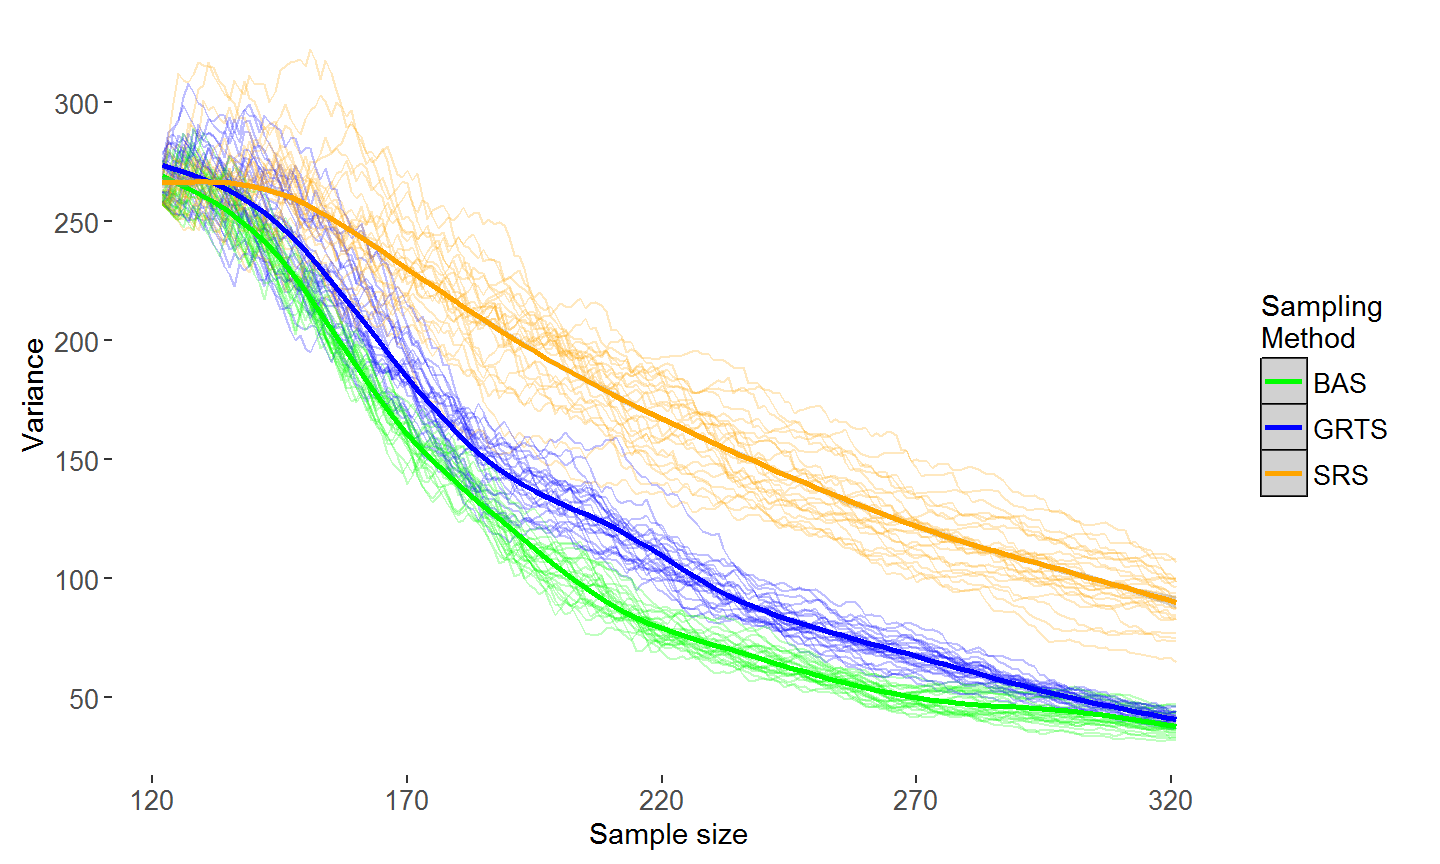
\includegraphics[scale = 0.5]{SpatialBalanceTier1}
	\caption{Results from a simulation study testing the spatial balance of 120 systematic points with BAS, GRTS, and Simple Random Sampling (SRS) points added on top.}
	\label{balance}
\end{figure}

\begin{figure}
	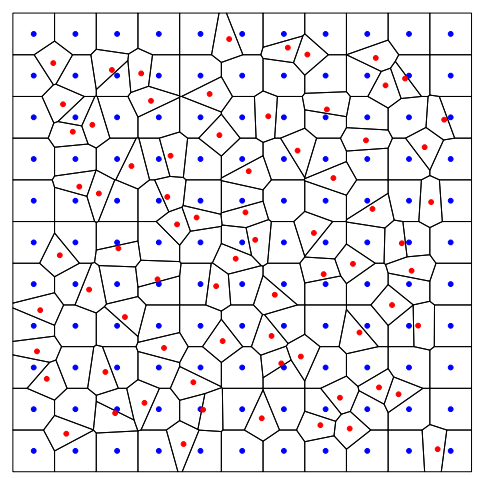
\includegraphics[scale = 0.5]{intense}
	\caption{Example of BAS Points being added to a systematic grid where blue is the existing points and red is BAS.}
	\label{voronoi}
\end{figure}

\begin{table}
	\begin{tabular}{c c c c c c c c c c c c}
		\hline
		& \multicolumn{10}{c}{Sample Occasion}\\ 
		\cline{2-11}
		Panel & 1 & 2 & 3 & 4 & 5 & 6 & 7 & 8 & 9 & 10 \\ \hline
		1 & X & X & X & X & X & X & X & X & X & X \\
		2 & X &   &  &X &   &   & X &   &  & X \\
		3 &   & X &  &  & X &   &   & X &  &   \\
		4 &   &   &  X  &   &   & X &   &  & X \\
		\hline
	\end{tabular} 
	\caption{Example of a panel design with revisit strategy of $[1-0,(1-2)^3]$.}
	\label{Panel}
\end{table}

\begin{figure}
	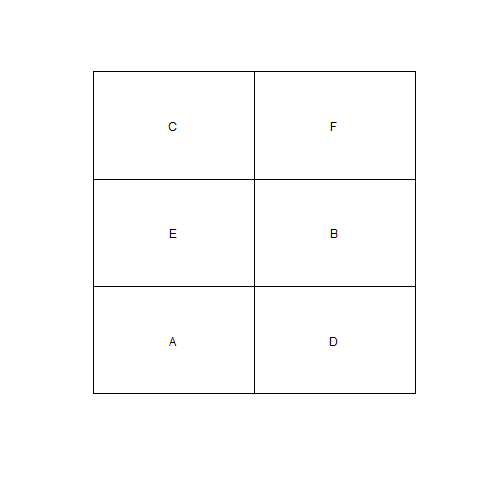
\includegraphics[scale = 0.5]{HaltonGrid}
	\caption{A Halton grid with $(2,3)$ co-prime base. The first six points in a sequence starting in B have the pattern (B,C,F,A,D,E).}
	\label{grid}
\end{figure}


\end{document}
